\documentclass{article}
\usepackage{graphicx}
\usepackage{hyperref}
\usepackage{minted}
\usepackage{spreadtab}
\usepackage[margin=1.25in]{geometry}
\graphicspath{ {../imgs/} }
\STautoround{3}
\title{Progetto ICON 21/22}
\author{Francesco Bottalico - 718330 \\ f.bottalico15@outlook.it}
\date{}

\begin{document}
\maketitle
\tableofcontents

\section{Progetto}
\paragraph{Introduzione.}
Lo scopo di questo progetto è costruire dei modelli di regressione per la
predizione di prezzi di alcune case, partendo da caratteristiche della casa e
del luogo dove si trova. Inoltre vengono confrontate le performance di modelli
allenati sul dataset originale e su un dataset esteso, al quale sono state
aggiunte alcune features attraverso query a \href{http://dbpedia.org}
{\textbf{DBpedia}}, quindi si vedrà se è possibile migliorare le predizioni 
dei prezzi attraverso l'integrazione di conoscenza proveniente dal web
semantico.

\subsection{Requisiti}
Il progetto è stato scritto interamente in \textbf{Python 3} e sono state usate
le seguenti librerie:
\begin{itemize}
	\itemsep0em
	\item numpy
	\item scikit-learn
	\item pandas
	\item sparqlwrapper
\end{itemize}

\subsection{Files}
La repository è organizzata nel seguente modo:
\begin{itemize}
	\itemsep0em
	\item \textbf{data:} in questa cartella sono contenuti i files .csv 
		contenenti il dataset (originale ed esteso)
	\item \textbf{src:} in questa cartella è presente il codice sorgente del
		progetto, in particolare:
		\begin{itemize}
		\itemsep0em
			\item \textbf{datasparql.py:} contiene il codice per effettuare le
				query a DBpedia
			\item \textbf{data\_preprocessing.py:} contiene il codice relativo
				al processing dei dati e per la gestione del dataset
			\item \textbf{models.py:} contiene il codice relativo alla
				costruzione dei vari modelli di apprendimento e gestisce il
				training ed il testing
		\end{itemize}
	\item \textbf{docs:} contiene la documentazione del progetto
	\item \textbf{img:} contiene la documentazione del progetto
\end{itemize}

\section{Analisi dei dati, processing e conoscenza dal web semantico}
Nel dataset originale (presente in \textit{data/data.csv}), sono presenti i
seguenti attributi:
\begin{enumerate}
	\itemsep0em
	\item \textbf{date:} data di rilevazione
	\item \textbf{price:} prezzo della casa
	\item \textbf{bedrooms:} numero di stanze da letto
	\item \textbf{bathrooms:} numero di bagni
	\item \textbf{sqft\_living:} dimensione della casa
	\item \textbf{sqft\_lot:} dimensione del terreno
	\item \textbf{floors:} numero di piani
	\item \textbf{waterfront:} se la casa è sul mare
	\item \textbf{view:} voto della vista
	\item \textbf{condition:} condizione della casa
	\item \textbf{sqft\_above:} dimensione della casa escluse stanze sotterranee
	\item \textbf{sqft\_basement:} dimensione di un eventuale piano sotterraneo
	\item \textbf{yr\_built:} anno di costruzione
	\item \textbf{yr\_renovated:} anno di ristrutturazione
	\item \textbf{street:} via
	\item \textbf{city:} città
	\item \textbf{statezip:} codice zip
	\item \textbf{country:} nazione
\end{enumerate}

\subsection{Estensione del dataset}
Nel file \textit{data/ext\_data.csv} è presente il dataset che è stato esteso
attraverso le query a DBpedia, le quali vengono effettuate nel modulo
\textbf{datasparql.py}, in particolare la funzione:
\begin{minted}[frame=single]{Python}
def citiesDensity(cities: list)
\end{minted}
permette di estrarre la densità abitativa di una lista di città. Invece la
funzione:
\begin{minted}[frame=single]{Python}
def citiesCoords(cities: list)
\end{minted}
permette di estrarre latitudine e longitudine delle città, questo permetterà di
sostituire la feature \textbf{city} con le features \textbf{lat} e
\textbf{long} e quindi rappresentare la città non come una categoria ma
attraverso valori numerici. Un altro vantaggio è che la predizione per una casa
in una città che non è presente nel set di training sarà più precisa grazie
all'uso di latitudine e longitudine. \\
La conoscenza proveniente dal web semantico permette quindi di aggiungere le
seguenti features:
\begin{itemize}
	\itemsep0em
	\item \textbf{lat:} latitudine
	\item \textbf{long:} longitudine
	\item \textbf{density:} densità di popolazione
\end{itemize}
La posizione della casa effettivamente influisce sul prezzo, mentre la densità
sembra influire meno, come si può vedere nella figura \ref{fig:cities}.
\begin{figure}[ht]
	\centering
	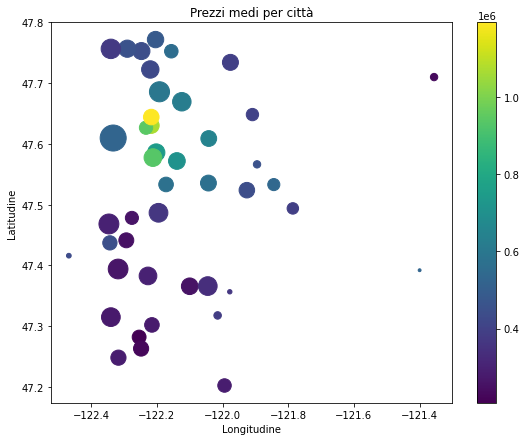
\includegraphics[scale=0.4]{cities}
	\label{fig:cities}
	\caption{Case raggruppate per città, il colore rappresenta il prezzo
	medio delle case, la grandezza del punto mostra la densità di popolazione.}
\end{figure}

\subsection{La classe Dataset}
Nel modulo \textbf{data\_preprocessing.py} sono presenti classi e metodi
relativi alla gestione del dataset, cioè caricamento da file system,
preprocessing e generazione dei set di training e testing.

La classe \textbf{Dataset} permette il caricamento del dataset da file system e
prova a caricare la relativa versione estesa (chiamata \textit{ext\_data.csv}),
se questa non viene trovata, allora vengono utilizzati i metodi presenti nel
modulo \textbf{datasparql.py} per effettuare le query e generare il dataset
esteso. Entrambe le versioni del dataset vengono esposte come attributi di
classe, rispettivamente denominate \textbf{original\_data} e
\textbf{extended\_data}.

\subsection{Gestione delle features}
Sul dataset vengono effettuate diverse operazioni:
\begin{description}
	\item[Elementi con prezzo nullo] Sono presenti 49 entry con prezzo uguale a
		zero, le quali devono essere rimosse.
		\begin{minted}{Python}
In [1]: data.price.value_counts()
Out[1]:
0.0          49
300000.0     42
400000.0     31
440000.0     29
450000.0     29
..
684680.0      1
609900.0      1
1635000.0     1
1339000.0     1
220600.0      1
Name: price, Length: 1741, dtype: int64
In [2]: data.drop(index=data[data.price == 0].index, inplace=True)
		\end{minted}
	\item[Feature selection] Alcune features devono essere rimosse, in
		particolare:
		\begin{description}
			\item[date] La data di rilevazione viene rimossa in quanto non da
				alcuna informazione aggiuntiva, infatti tutte le date sono
				ristrette ad un breve periodo di tempo.
			\item[street] L'indirizzo della casa viene rimosso.
			\item[country] La nazione viene rimossa in quanto tutte le case
				presenti nel dataset si trovano negli USA.
			\item[waterfront] Solo 33 case su 4600 hanno questa feature
				impostata su 1, quindi l'attributo viene rimosso.
		\end{description}
		Tracciando la matrice di correlazione tra le feature e il prezzo della
		casa, e rimuovendo quelle poco correlate si hanno peggioramenti nella
		predizione, quindi non è stata rimossa nessun altra feature.
		\begin{figure}[ht]
			\centering
			\begin{minipage}{0.48\textwidth}
				\centering
				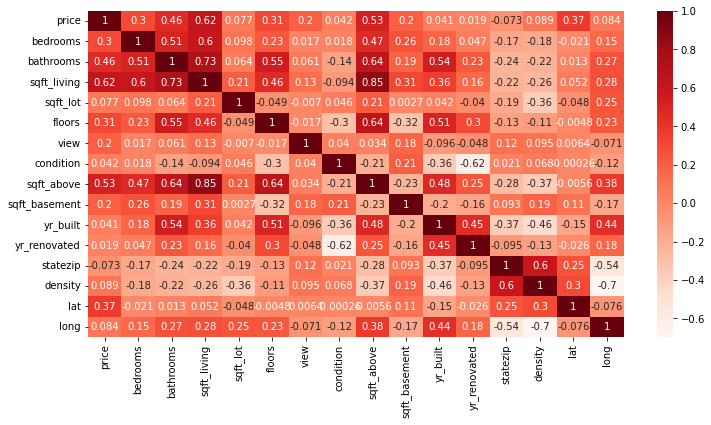
\includegraphics[width=\textwidth]{correlazione.png}
				\caption{Matrice di correlazione tra le features}
			\end{minipage}
			\hfill
			\begin{minipage}{0.48\textwidth}
				\centering
				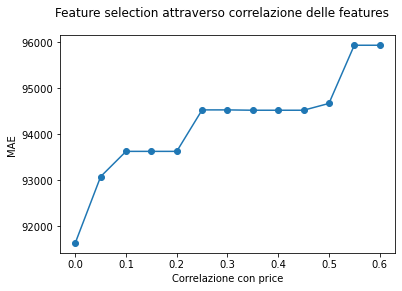
\includegraphics[width=\textwidth]{selection.png}
				\caption{Andamento dell'errore assoluto medio delle predizioni
				alla rimozione di feature con correlazione minore di un dato
				valore}
			\end{minipage}
			\label{fig:selection}
		\end{figure}
	\item[Anno di ristrutturazione] la feature \textbf{yr\_renovated} indica
		l'anno di ristrutturazione della casa, se questa non è mai stata
		ristrutturata il valore sarà uguale a zero. Per evitare di avere valori
		nulli, questo valore viene sostituito con il valore della feature
		\textbf{yr\_built}, cioé $yr\_renovated = yr\_built$ se la casa non è
		mai stata ristrutturata.
		\begin{minted}{Python}
In [3]: data.yr_renovated = data[["yr_built", "yr_renovated"]].max(axis=1)
		\end{minted}
	\item[Rimozione outliers] Vengono rimossi tutti gli elementi del dataset
		che contengono almeno un outlier in una feature, cioè se lo zscore di
		un attributo è maggiore di 2.5 o minore di -2.5 (sono escluse le
		feature \textbf{lat}, \textbf{long} e \textbf{density})
		\begin{minted}{Python}
In [4]: data[(abs(zscore(data.loc[:, :"yr_renovated"])) < 2.5).all(axis=1)]
		\end{minted}
	\item[Standardizzazione] Alcuni modelli di regressione che verranno
		utilizzati \\per effettuare le predizioni sul prezzo funzionano meglio
		se gli elementi del dataset vengono standardizzati, cioè se i valori
		delle feature vengono trasformati nei valori di una distribuzione
		normale standard. Questa operazione viene effettuata prima del training
		dei modelli nel modulo \textbf{models.py}, grazie alla classe
		\textbf{StandardScaler()} della libreria \\
		\textbf{sklearn.preprocessing}
	\item[One hot encoding] Eventuali feature categoriche vengono codificate\\
		utilizzando il one hot encoding (come per la standardizzazione questa
		operazione viene effettuata nel modulo \textbf{models.py} prima del
		training.
\end{description}
Tutte queste operazioni vengono eseguite dalla funzione:
\mint[frame=single]{Python}|def _data_preprocess(data, statezip=False)|

\subsection{Splitting del dataset}
Sono infine presenti due metodi per generare il set di training e di testing a
partire dal dataset completo.

\subsubsection{Equal splitting}
\label{sec:eqsplit}
La prima funzione è un wrapper per la funzione di splitting
\textbf{train\_test\_split()} del modulo \\\textbf{sklearn.model\_selection},
che prima di effettuare lo splitting esegue il preprocessing dei dati.
\mint[frame=single]{Python}|def train_test_equal_split(data, tr_size=0.8, ext=False, random_state=None)|
\begin{description}
	\item[data] Dataset sul quale effettuare lo splitting.
	\item[tr\_size] Dimensione del set di training.
	\item[ext] True se viene passato il dataset esteso, permette di eliminare
		la feature \textbf{city} che sarà sostituita da \textbf{lat},
		\textbf{long} e \textbf{density}.
	\item[random\_state] Per risultati riproducibili.
\end{description}

\subsubsection{Train e test con città differenti}
\label{sec:diffsplit}
La seconda funzione permette di simulare il caso in cui nel set di testing
siano presenti città differenti rispetto al set di training, per valutare le
performance dei vari modelli di regressione in questo scenario e quindi
vedere se l'integrazione della conoscenza dal web semantico permette la
creazione di modelli più performanti.
\mint[frame=single]{Python}|def train_test_diffcities_split(data, tr_size=0.8, ext=False, random_state=None)|

\section{Modelli di regressione}
\label{sec:regressionintro}
Per effettuare le predizioni sul prezzo delle case sono stati usati diversi
modelli di regressione lineare e non, al fine di confrontare i risultati dei
vari modelli e trovare i più performanti. Questi modelli sono creati, allenati
e testati nel modulo \textbf{models.py}, dove viene anche effettuata la model
selection per trovare dei valori ottimali per gli iperparametri, attraverso
una K-fold cross validation ($k = 5$). Ciascun modello viene allenato e testato
quattro volte:
\begin{enumerate}
	\item La prima volta i modelli sono allenati sul dataset originale, il
		quale viene diviso in training e testing set utilizzando la funzione
		\textbf{train\_test\_equal\_split()}.
	\item La seconda volta si utilizza il dataset esteso utilizzando la
		medesima funzione di splitting. A questo punto sarà possibile
		confrontare i risultati delle predizioni allenando uno stesso modello
		allenato però con i diversi dataset.
	\item Successivamente i modelli vengono allenati con il dataset originale
		simulando la situazione in cui nel testing vengono incontrati case
		in città mai incontrate durante il training (viene utilizzata la
		funzione \textbf{train\_test\_diffcities\_split()}).
	\item Infine utilizzando la funzione di splitting precedente, i
		modelli sono allenati sul dataset esteso, così da confrontare le
		performance tra dataset originale ed esteso in questo scenario.
\end{enumerate}
Per ottenere risultati confrontabili in ogni testing, viene passato lo stesso
seed al parametro \textbf{random\_state} ad ogni chiamata della funzione di
splitting, così da ottenere la medesima divisione del dataset.

\subsection{Apprendimento Supervisionato}
Per primi vengono allenati dei modelli (lineari e non) che utilizzando
algoritmi di apprendimento supervisionato, in particolare:
\begin{itemize}
	\itemsep0em
	\item Rete neurale (multilayer perceptron)
	\item Regressione lineare con regolarizzazione L1
	\item Regressione lineare con regolarizzazione L2
	\item Decision tree
	\item Random forest
	\item Support vector machine
\end{itemize}
Per ciascuno di questi modelli vengono cercati degli iperparametri ottimali
utilizzando la classe \textbf{GridSearchCV()} fornita dal modulo
\textbf{sklearn.model\_selection}.
La model selection, il training ed il testing di ciascun modello viene
effettuato dalla funzione \textbf{train\_eval()}.

\subsubsection{Rete neurale}
Per la rete neurale viene effettuata la model selection su diversi parametri
quali: algoritmo di ottimizzazione, numero di neuroni e strati e parametro per
la regolarizzazione L2 ($\alpha$ nella formula \ref{eq:nn}). La funzione
\ref{eq:nn} mostra il valore che la rete neurale cerca di ottimizzare.
\begin{equation}
	Loss(y, \hat{y}, W)=\frac{1}{2}(\hat{y}-y)^2 + \alpha\|W\|^2_2
	\label{eq:nn}
\end{equation}
\begin{figure}[ht]
	\centering
	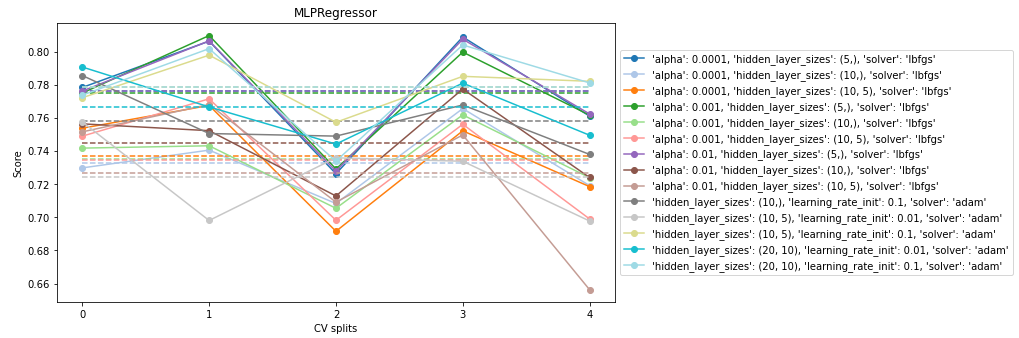
\includegraphics[width=0.9\textwidth]{nncv.png}
	\caption{Andamento dello score sui vari fold della cross validation dati
	diversi valori per gli iperparametri. le rette tratteggiate indicano il
	valore medio.}
\end{figure}

\subsubsection{Regressione lineare}
Gli iperparametri che vengono stimati dalla cross validation sono il learning
rate, il suo metodo di aggiornamento ed il parametro di regolarizzazione
$\alpha$.
\paragraph{Regolarizzazione L1}
In questo caso viene utilizzata la discesa di gradiente stocastica per
ottimizzare la funzione \ref{eq:sgd1}.
\begin{equation}
	Loss(y, \hat{y}, W)=\frac{1}{2}(\hat{y}-y)^2 + \alpha\|W\|
	\label{eq:sgd1}
\end{equation}
\paragraph{Regolarizzazione L2} La funzione che viene ottimizzata in questo
caso è la stessa della rete neurale (formula \ref{eq:nn}).
\begin{figure}[ht]
	\centering
	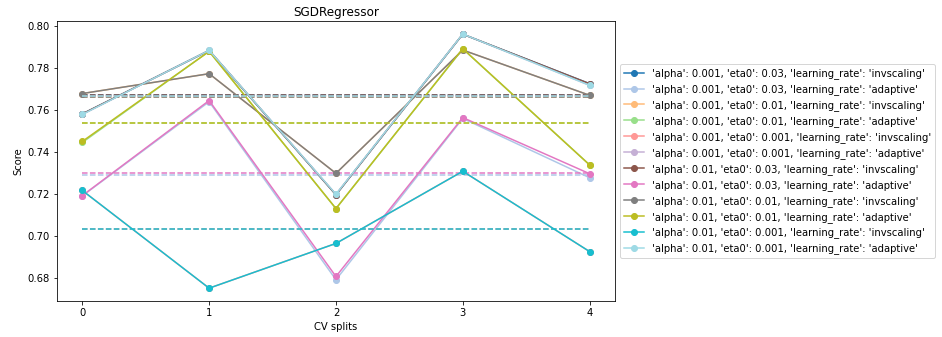
\includegraphics[width=0.75\textwidth]{lassocv.png}
	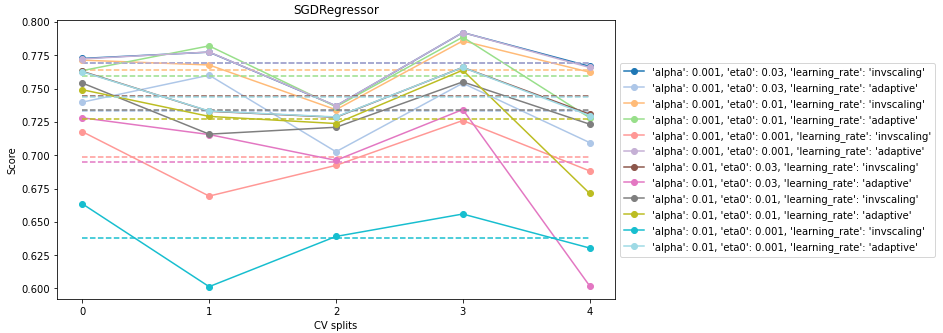
\includegraphics[width=0.75\textwidth]{ridgecv.png}
	\caption{Score delle cross validation per la model selection dei modelli
	di regressione lineare con regolarizzazione L1 (sopra) ed L2 (sotto).}
\end{figure}

\subsubsection{Decision tree}
Per il decision tree la cross validation viene utilizzata per stimare parametri
quali la massima profondità dell'albero ed il numero minimo di sample che una
foglia può contenere.
\begin{figure}[ht]
	\centering
	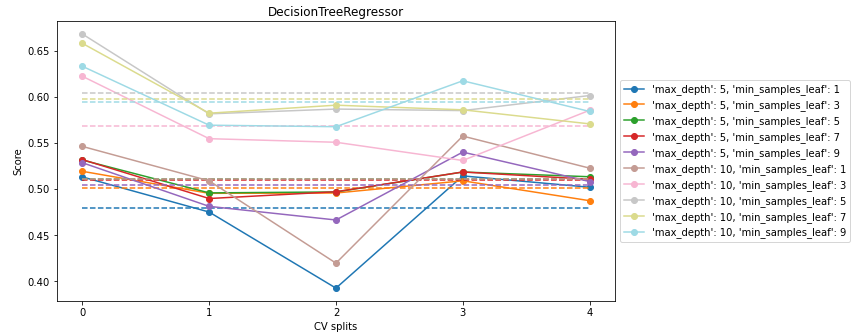
\includegraphics[width=0.9\textwidth]{treecv.png}
	\caption{Score delle cross validation per la model selection del decision
	tree.}
\end{figure}

\subsubsection{Random forest}
Per la random forest vengono allenati 100 decision trees, gli iperparametri
stimati attraverso la cross validation sono la profondità massima degli alberi
ed il numero massimo di feature prese in considerazione durante il training.
\begin{figure}[ht]
	\centering
	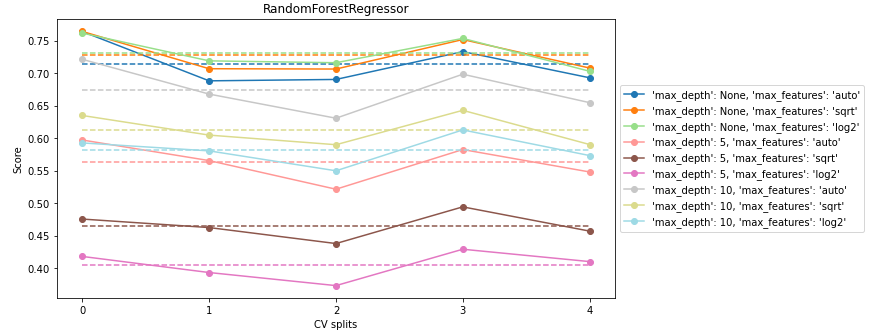
\includegraphics[width=0.9\textwidth]{ranfcv.png}
	\caption{Score delle cross validation per la model selection del decision
	tree.}
\end{figure}

\subsubsection{Support vector machine}
Nel caso della SVM vengono provate diverse funzioni kernel (per il kernel
polinomiale si provano diversi gradi) e alcuni valori per il parametro per la
regolarizzazione C (che è inversamente proporzionale alla forza della
regolarizzazione).
\begin{figure}[ht]
	\centering
	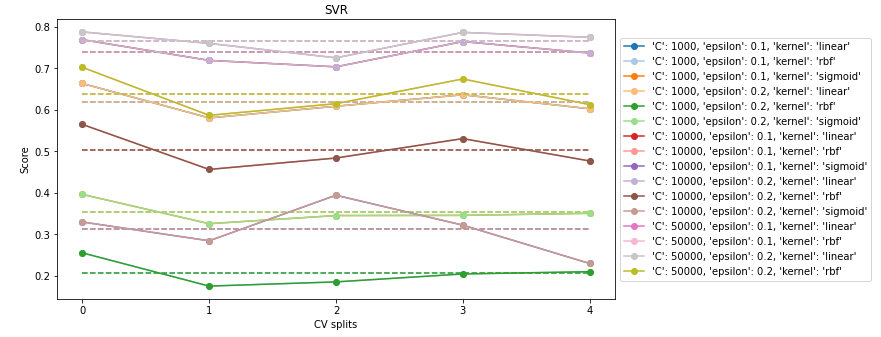
\includegraphics[width=0.9\textwidth]{svmcv.png}
	\caption{Score delle cross validation per la model selection della support
	vector machine.}
\end{figure}

\subsection{Clustering}
\label{sec:clustering}
Possono essere usati algoritmi di apprendimento non supervisionato come il
K-means, combinati con i precedenti modelli, per migliorare ulteriormente le
performance.\\
L'idea è quella di dividere il training set in cluster e di allenare su ogni
cluster un modello supervisionato indipendente da quello degli altri cluster.
Per effettuare una predizione il dato viene prima assegnato ad un cluster, per
poi utilizzare il relativo modello supervisionato.
Il clustering può essere effettuato in due modi:
\begin{enumerate}
	\item Il K-means viene allenato su tutte le feature dei dati, anche se
		questi hanno un'alta dimensionalità. In questo caso il miglior valore
		per k sembra essere $k=2$ come si vede nella figura a sinistra,
		anche se i dati non sono molto divisibili e quindi questo approccio
		probabilmente non migliorerà molto la precisione dei modelli.
		\begin{figure}[ht]
			\centering
			\begin{minipage}{0.48\textwidth}
				\centering
				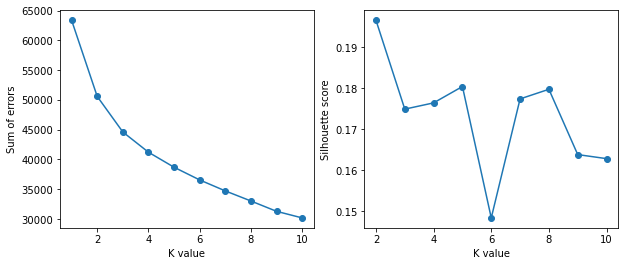
\includegraphics[width=\textwidth]{kselection1.png}
				\caption{Andamento dell'errore all'aumentare di k nel caso (1)}
			\end{minipage}
			\hfill
			\begin{minipage}{0.48\textwidth}
				\centering
				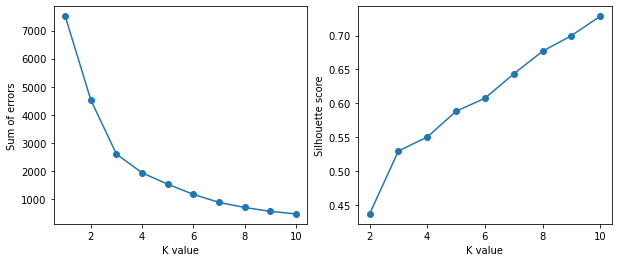
\includegraphics[width=\textwidth]{kselection2.png}
				\caption{Andamento dell'errore all'aumentare di k nel caso (2)}
			\end{minipage}
		\end{figure}
	\item Il K-means viene allenato utilizzando solo le feature latitudine
		e longitudine (in caso di utilizzo del dataset esteso). In questo caso
		si prende in considerazione il rapporto che esiste tra luogo della casa
		ed il suo prezzo (come visto nella figura \ref{fig:cities} a pagina
		\pageref{fig:cities}). In questo caso il valore ottimale per k sembra
		essere $k=3$ come si può vedere dall'andamento delle curve nella
		figura a destra.
\end{enumerate}

La seguente funzione divide il training set in k cluster e su ciascuno di
questi esegue il training di ogni modello passato in input (viene creata una
copia per cluster), inoltre esegue il testing assegnando il sample al relativo
cluster ed utilizza per la predizione il relativo modello.
\begin{minted}[frame=single]{Python}
def train_eval_cluster(models, train, test, preproc, k, models_per_cl=False, 
                       latlong=True, draw=False):
\end{minted}
\begin{description}
	\item[models] Lista dei modelli da allenare, viene effettuatuata una copia
		per ogni cluster cosi da avere ogni modello allenato su ogni cluster.
	\item[train] Dataset di training
	\item[test] Dataset di testing
	\item[preproc] Funzione per trasformare i dati prima del training.
	\item[k] Numero di cluster per il K-means
	\item[models\_per\_cl] Se impostato su \textbf{True} il parametro models
		deve essera una lista di k modelli, l'i-esimo modello della lista verrà
		utilizzato sull'i-esimo cluster. Questa opzione può essere utile per
		combinare modelli differenti ed avere in alcuni casi prestazioni
		migliori.
	\item[latlong] Se applicare il K-means su tutte le feature o solamente su
		latitudine e longitudine.
	\item[draw] Se mostrare i grafici del clustering.
\end{description}
\newpage

\section{Confronto dei modelli}
Come spiegato nella sezione \ref{sec:regressionintro}, i modelli verranno
allenati quattro volte, per poter confrontare le differenze di prestazioni tra
i modelli allenati sul dataset originale e quelli allenati sul dataset esteso,
nei due scenari già spiegati.

\subsection{Equal splitting}
Di seguito sono confrontati i risultati dei vari modelli allenati prima sul
dataset originale e poi su quello esteso, utilizzando come funzione di
splitting del dataset il metodo \textbf{train\_test\_equal\_split()} (spiegato
nella sezione \ref{sec:eqsplit}). Tra gli stimatori utilizzati, oltre
a quelli presentati in precedenza, è stato aggiunto uno stimatore \textit{Dummy}
(che predice sempre il valore medio) per confronto.
\begin{table}[ht]
	\centering
	\begin{spreadtab}{{tabular}{c|c|c|c|c|c|c|r|}}
		\cline{2-8}
		& @ \multicolumn{3}{|c|}{Original data} & @ \multicolumn{3}{c|}{Extended data} & \\
		\cline{2-7}
		& @ R2 & @ RMSE & @ MAE & @ R2 & @ RMSE & @ MAE & @ decr. MAE\\
		\hline
		@ \multicolumn{1}{|c|}{Dummy} & -0.003 & 253592.36 & 191642.73 &
		-0.003 & 253592.36 & 191642.73 & \textbf{:={[-4,0]*100/[-1,0]-100}}\%\\
		\hline
		@ \multicolumn{1}{|c|}{Rete neurale} & 0.835 & 102802.54 & 67716.71 &
		0.843 & 100257.86 & 66375.14 & \textbf{:={[-4,0]*100/[-1,0]-100}}\%\\
		\hline
		@ \multicolumn{1}{|c|}{Lasso} & 0.820 & 107530.43 & 71892.61 &
		0.818 & 107884.67 & 72514.84 & \textbf{:={[-4,0]*100/[-1,0]-100}}\%\\
		\hline
		@ \multicolumn{1}{|c|}{Ridge} & 0.811 & 109967.49 & 73629.67 &
		0.812 & 109665.55 & 72766.01 & \textbf{:={[-4,0]*100/[-1,0]-100}}\%\\
		\hline
		@ \multicolumn{1}{|c|}{Decision tree} & 0.688 & 141346.10 & 100310.09 &
		0.711 & 136167.39 & 91516.67 & \textbf{:={[-4,0]*100/[-1,0]-100}}\%\\
		\hline
		@ \multicolumn{1}{|c|}{Random forest} & 0.772 & 120975.81 & 77201.70 &
		0.785 & 117388.42 & 74131.08 & \textbf{:={[-4,0]*100/[-1,0]-100}}\%\\
		\hline
		@ \multicolumn{1}{|c|}{SVM} & 0.800 & 113336.14 & 70691.88 &
		0.796 & 114286.55 & 71563.63 & \textbf{:={[-4,0]*100/[-1,0]-100}}\%\\
		\hline
	\end{spreadtab}
	\label{tab:eq}
	\caption{Risultati predizioni usando la funzione di equal splitting.}
\end{table}

Non si notano sostanziali miglioramenti allenando i modelli con il dataset
esteso, solamente le predizioni effettuate con stimatori basati su alberi di
decisione subiscono un buon decremento del \textit{mean average error}, in
particolare il decision tree ha un miglioramento di quasi il 10\%.
Questo accade probabilmente perchè le feature introdotte nel dataset esteso
permettono di splittare meglio i dati rispetto all'utilizzo di una feature
categorica.

\begin{figure}[ht]
	\centering
	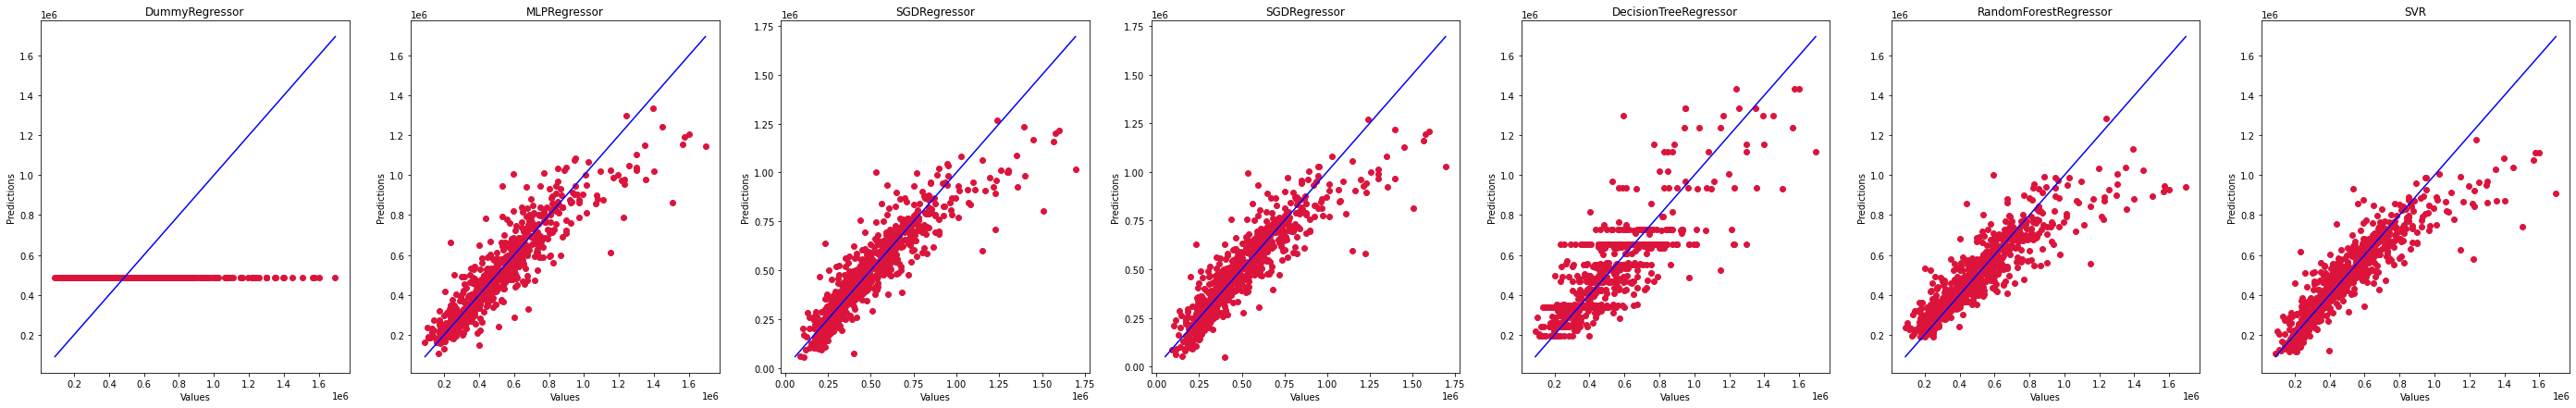
\includegraphics[width=\textwidth]{predoriginal.png}
	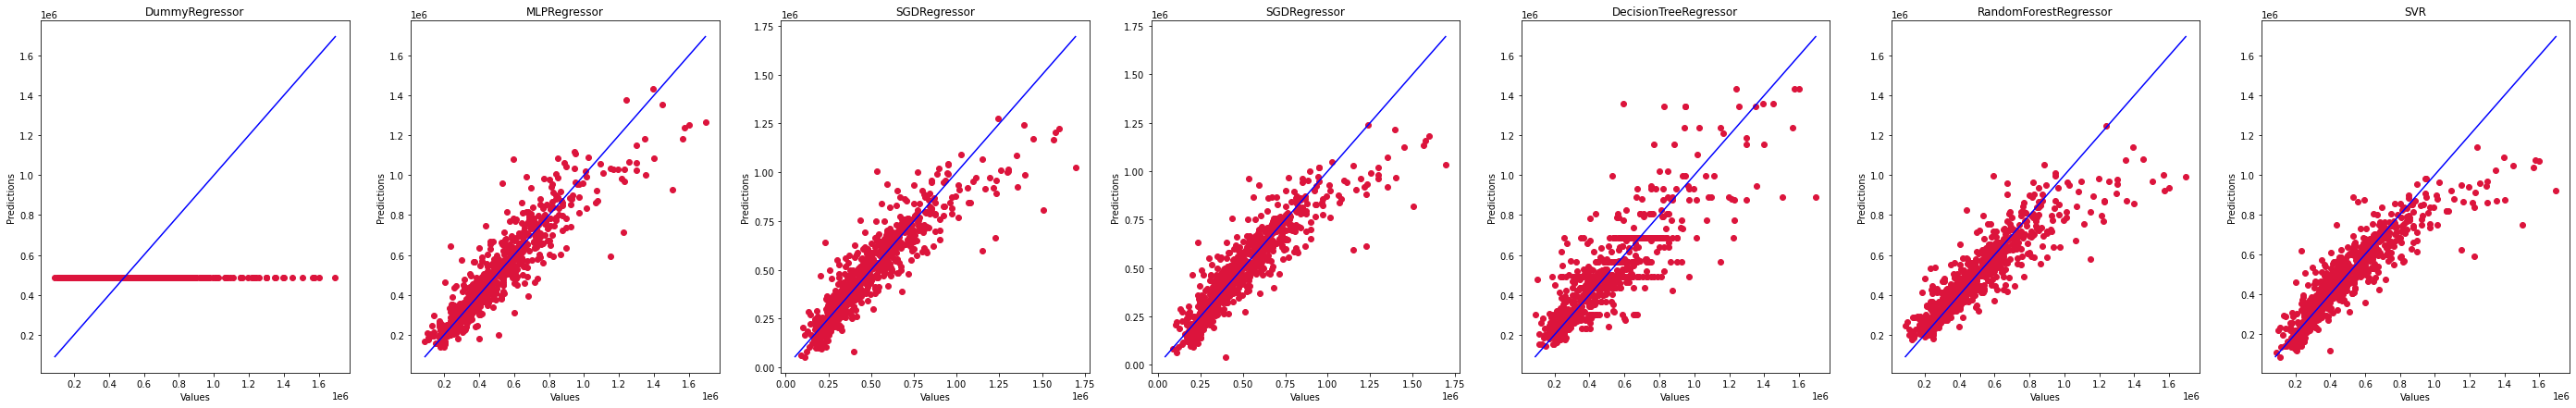
\includegraphics[width=\textwidth]{predextended.png}
	\caption{Grafici predizione/valore attuale per ogni modello, sopra allenati
	con il dataset originale, sotto con quello esteso. Si nota anche attraverso
	il grafico il miglioramento nel decision tree.}
\end{figure}

\subsubsection{Clustering}
Possiamo ulteriormente migliorare le performance dei modelli allenati con il
dataset esteso attraverso l'utilizzo del clustering come spiegato nella sezione
\ref{sec:clustering}.
\begin{table}[ht]
	\small
	\centering
	\begin{tabular}{c|c|c|c|c|c|c|r|}
		\cline{2-8}
		& \multicolumn{2}{|c}{\textbf{Cluster 1} (304/751)}
		& \multicolumn{2}{|c|}{\textbf{Cluster 2} (206/751)}
		& \multicolumn{2}{c|}{\textbf{Cluster 3} (241/751)} & \\
		\cline{2-7}
		& RMSE & MAE & RMSE & MAE & RMSE & MAE & Tot MAE \\
		\hline
		\multicolumn{1}{|c|}{Rete neurale} & 120621.89 & 84109.27 & 54167.91 &
		36626.51 & 107014.35 & 70194.79 & \textbf{66619.47}\\
		\hline
		\multicolumn{1}{|c|}{Lasso}	& 122742.48 & 85282.69 & 53754.36 &
		37012.46 & 110568.84 & 72466.94 & \textbf{67929.47}\\
		\hline
		\multicolumn{1}{|c|}{Ridge} & 126733.21 & 86639.71 & 54087.48 &
		36824.57 & 111961.88 & 73232.25 & \textbf{68672.84}\\
		\hline
		\multicolumn{1}{|c|}{Decision tree} & 175090.90 & 125769.12 & 71349.57 &
		48866.83 & 139656.11 & 86026.76 & \textbf{91921.21}\\
		\hline
		\multicolumn{1}{|c|}{Random forest} & 133296.10 & 92910.04 & 57140.54 &
		40125.23 & 130805.02 & 76968.65 & \textbf{73315.43}\\
		\hline
		\multicolumn{1}{|c|}{SVM} & 120161.80 & 82193.35 & 55079.35 &
		36726.16 & 117846.77 & 75034.62 & \textbf{67424.37}\\
		\hline
	\end{tabular}
	\caption{Risultati delle predizioni combinando apprendimento supervisionato
	e K-means.}
\end{table}
\\
Tra parentesi accanto al numero del cluster sono indicati il numero di esempi
classificati come appartenenti al cluster sul totale degli esempi di test. 
La colonna "Tot MAE" non è altro che la media tra tutti i cluster calcolata
come:
\begin{equation}
	\frac{\sum_{i=1}^k MAE_i \cdot |Cluster_i|}{\sum_{i=1}^k |Cluster_i|}
\end{equation}
In questo caso riscontriamo qualche piccolo miglioramento negli stimatori
\textbf{Lasso}, \textbf{Ridge} e \textbf{SVM}. Inoltre si può notare come
alcuni stimatori funzionano meglio di altri su specifici cluster, si potrebbe
quindi pensare di combinare modelli differenti su cluster diversi per
massimizzare le performance (vedere la sezione \ref{sec:clustering}).
\begin{figure}[ht]
	\centering
	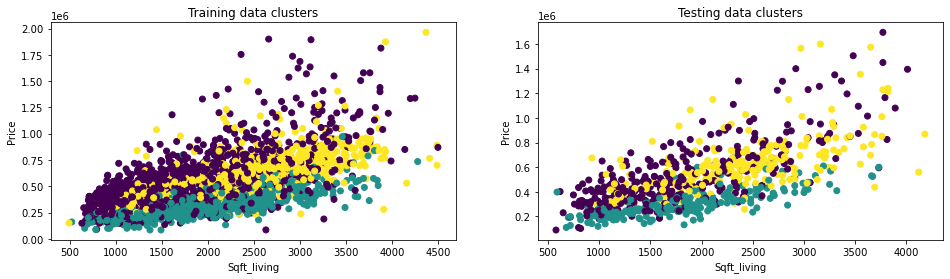
\includegraphics[width=\textwidth]{clustereq.png}
	\caption{I tre cluster distribuiti sul training e testing set.}
\end{figure}

\subsection{Train e test con città differenti}
Utilizzando come funzione di splitting \textbf{train\_test\_diffcities\_split()}
simuliamo lo scenario nel quale durante il testing si incontrano case in città
non presenti nel set di training (la dimensione dei set è sempre 80\% training,
 20\% test). I risultati delle predizioni sono i seguenti.
\begin{table}[ht]
	\centering
	\begin{spreadtab}{{tabular}{c|c|c|c|c|c|c|r|}}
		\cline{2-8}
		& @ \multicolumn{3}{|c|}{Original data} & @ \multicolumn{3}{c|}{Extended data} & \\
		\cline{2-7}
		& @ R2 & @ RMSE & @ MAE & @ R2 & @ RMSE & @ MAE & @ decr. MAE\\
		\hline
		@ \multicolumn{1}{|c|}{Dummy} & -0.000 & 241153.04 & 189087.16
		& -0.000 & 241153.04 & 189087.16 & \textbf{:={[-4,0]*100/[-1,0]-100}}\%\\
		\hline
		@ \multicolumn{1}{|c|}{Rete neurale} & 0.117 & 226651.86 & 182441.63
		& 0.392 & 188103.04 & 141451.75 & \textbf{:={[-4,0]*100/[-1,0]-100}}\%\\
		\hline
		@ \multicolumn{1}{|c|}{Lasso} & 0.477 & 174465.26 & 137111.43
		& 0.600 & 152593.23 & 109693.36 & \textbf{:={[-4,0]*100/[-1,0]-100}}\%\\
		\hline
		@ \multicolumn{1}{|c|}{Ridge} & 0.487 & 172658.18 & 134693.90
		& 0.600 & 152514.45 & 109608.88 & \textbf{:={[-4,0]*100/[-1,0]-100}}\%\\
		\hline
		@ \multicolumn{1}{|c|}{Decision tree} & -0.211 & 265360.75 & 197765.79
		& 0.542 & 163191.47 & 108231.19 & \textbf{:={[-4,0]*100/[-1,0]-100}}\%\\
		\hline
		@ \multicolumn{1}{|c|}{Random forest} & 0.368 & 191684.83 & 149244.86
		& 0.630 & 146678.88 & 104214.31 & \textbf{:={[-4,0]*100/[-1,0]-100}}\%\\
		\hline
		@ \multicolumn{1}{|c|}{SVM} & 0.439 & 180650.80 & 136976.35
		& 0.599 & 152661.49 & 106088.53 & \textbf{:={[-4,0]*100/[-1,0]-100}}\%\\
		\hline
	\end{spreadtab}
	\label{tab:diff}
\end{table}

In questo scenario il \textit{mean average error} aumenta, quindi la qualità
delle predizioni diminuisce sostanzialmente rispetto ai risultati precedenti.
In questo caso però i modelli allenati con il dataset esteso funzionano
notevolmente meglio rispetto a quelli allenati con il dataset originale.

\subsubsection{Clustering}
Anche in questo caso possiamo combinare il clustering con questi stimatori per
migliorare la qualità delle predizioni.
\begin{table}[ht]
	\small
	\centering
	\begin{tabular}{c|c|c|c|c|c|c|r|}
		\cline{2-8}
		& \multicolumn{2}{|c}{\textbf{Cluster 1} (95/671)}
		& \multicolumn{2}{|c|}{\textbf{Cluster 2} (354/671)}
		& \multicolumn{2}{c|}{\textbf{Cluster 3} (222/671)} & \\
		\cline{2-7}
		& RMSE & MAE & RMSE & MAE & RMSE & MAE & Tot MAE \\
		\hline
		\multicolumn{1}{|c|}{Rete neurale} & 329103.37 & 265676.82 & 138318.85
		& 106167.82 & 64009.57 & 45005.89 & \textbf{108515.67} \\
		\hline
		\multicolumn{1}{|c|}{Lasso} & 246069.36 & 209740.80 & 147408.77
		& 100309.35 & 65457.82 & 46995.73 & \textbf{98163.84} \\
		\hline
		\multicolumn{1}{|c|}{Ridge} & 241350.01 & 205236.32 & 147258.72
		& 100224.03 & 65334.73 & 46834.07 & \textbf{97427.60} \\
		\hline
		\multicolumn{1}{|c|}{Decision tree} & 279222.81 & 195405.96 & 177526.54
		& 125350.35 & 83347.69 & 57663.32 & \textbf{112874.59} \\
		\hline
		\multicolumn{1}{|c|}{Random forest} & 231919.25 & 176273.30 & 156945.97
		& 107479.84 & 68201.17 & 44938.32 & \textbf{96527.77} \\
		\hline
		\multicolumn{1}{|c|}{SVM} & 162850.36 & 123706.76 & 141990.15
		& 99907.89 & 64456.98 & 42933.31 & \textbf{84427.32} \\
		\hline
	\end{tabular}
	\caption{Risultati delle predizioni combinando apprendimento supervisionato
	e K-means.}
\end{table}
\\
Quasi tutti i modelli traggono benefici dall'uso del clustering, in particolare
la \textbf{SVM} che passa da un \textit{mean average error} di circa 106000 ad uno di
84400.
\begin{figure}[ht]
	\centering
	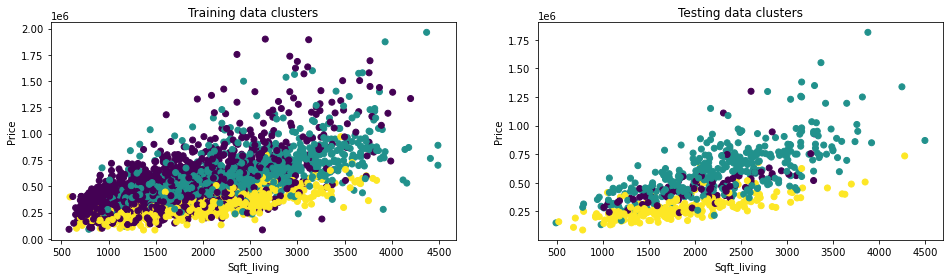
\includegraphics[width=\textwidth]{clusterdiff.png}
	\caption{I tre cluster distribuiti sul training e testing set.}
\end{figure}
\end{document}
